\documentclass[10pt,conference,compsocconf]{IEEEtran}

%\usepackage{times}
%\usepackage{balance}
\usepackage{amsmath}
\usepackage{url}
\usepackage{graphicx}
\usepackage{subfig}
\usepackage[pdftex]{hyperref}
\usepackage[utf8]{inputenc}

\usepackage{tikz}
\usetikzlibrary{shapes,arrows}

\begin{document}
\title{Inpainting with controlled frequency suppression in the Fourier domain}

\author{
  Group: NoobzRockz\\
  Patrick Bänziger, Kaspar Etter, Jan Rüegg\\
  Department of Computer Science, ETH Zurich, Switzerland
}

\maketitle

\begin{abstract}
This paper presents a new approach to the problem of inpainting, that is recovering of lost image information. In comparison with the submissions of our peers, we have designed a very efficient algorithm that does not fall behind other solutions in terms of accuracy. By suppressing weak frequencies in the Fourier domain, we attempt to recover the intrinsic signal of the image. Since we choose the optimal threshold using a random validation set, our method performs particularly well for the reconstruction of edges.
\end{abstract}

\section{Introduction}
Inpainting is about reconstructing the missing spots of an image by guessing the correct values. The quality of such a restoration method can be evaluated by masking an image and comparing the reconstruction with the original.\\
Our approach is based on the assumption that (natural) images have some underlying characteristic that can be distinguished from noise. We initialize our reconstructed image with what we call Gaussian interpolation: Using MATLAB's filtering function, we compute a weighted sum over all the neighboring pixels that are known. This reconstruction introduces noise compared to the original image. The hope is that this noise is weak enough compared to the real signal, that we want to get rid of it. We do so by dividing the image into patches and analyzing these in the Fourier space, removing the weak frequencies that (hopefully) capture this noise and thereby recovering the intrinsic signal.\\
We repeat this procedure with the newly determined values until the error of a randomly chosen validation set converges or the maximum number of iterations is reached. This validation set consists of some of known pixels given to the algorithm, that are removed before starting the reconstruction. In order to determine the  threshold for suppressing weaker frequencies, this validation set (for which we know the correct values) can be used as an error measure.

\section{Methods}
\subsection{Related work}
Without knowing in depth the broad field of research about inpainting (also known as image interpolation), we were not able to find papers covering similar concepts as ours. Most methods are based on partial differential equations or some form of texture synthesis.

\subsection{New approach}

% Define block styles
\tikzstyle{decision} = [diamond, draw, fill=blue!20, 
    text width=4.5em, text badly centered, inner sep=0pt]

\tikzstyle{block} = [rectangle, draw, fill=blue!20, 
    text width=7em, text centered, rounded corners, minimum height=3em]

\tikzstyle{line} = [draw, -latex']

\tikzstyle{cloud} = [draw, ellipse,fill=red!20,
    minimum height=2em]
    
\begin{figure}
\begin{tikzpicture}[node distance = 1.5cm, auto]
  % Place nodes
  \node [cloud] (node1) {Start};
  \node [block, right of=node1, node distance = 3.1cm] (node2) {Remove validation set};
  \node [block, below of=node2] (node3) {Frame image};
  \node [block, below of=node3] (node4) {Gaussian interpolation};
  \node [decision, below of=node4, node distance = 1.8cm] (node5) {Iterative?};
  \node [block, right of=node5, node distance = 3.1cm, fill=green!20] (node6) {Find best threshold};
  \node [block, below of=node6, fill=green!20, node distance = 1.8cm] (node7) {Reset known values except validation set};

  \node [block, left of=node5, node distance = 3.1cm] (node8) {Find best threshold};
  \node [block, below of=node8] (node9) {Gaussian interpolation on original data};
  \node [block, below of=node9] (node10) {Apply best threshold};

  \node [block, right of=node10, node distance = 3.1cm] (node11) {Unframe image};
  \node [block, below of=node11] (node12) {Reset known values};
  \node [cloud, right of=node12, node distance = 3.1cm] (node13) {End};

  % Draw edges
  \path [line] (node1) -- (node2);
  \path [line] (node2) -- (node3);
  \path [line] (node3) -- (node4);
  \path [line] (node4) -- (node5);
  \path [line] (node5) -- node[above]{yes} (node6);
  \path [line] (node5) -- node[above]{no} (node8);

  \draw [->] (node6) to [bend left=20] (node7);
  \draw [->] (node7) to [bend left=20] (node6);

  \path [line] (node8) -- (node9);
  \path [line] (node9) -- (node10);
  \path [line] (node10) -- (node11);
  \path [line] (node11) -- (node12);
  \path [line] (node12) -- (node13);

  \path [line] (node7) |- (node11);
\end{tikzpicture}
\caption{Our newly proposed algorithm as a flowchart.}
\label{flowchart}
\end{figure}

As outlined in the introduction, we combined several ideas for obtaining an inpainting algorithm that provides both good results and fast performance. The input of our algorithm is the image to be restored together with a mask that indicates its unknown spots.\\
Before entering the iterative part of our algorithm, the following three steps are performed (as seen in figure \ref{flowchart}):
\begin{enumerate}
\item In order to guide the elimination of frequencies by finding the optimal threshold (as described below), we first remove additional pixels from the image and use them as the validation set. The fraction of additional pixels to be removed is a global parameter, which we optimized using gradient descent (as explained in section \ref{gradient_descent}).
\item Our reduction in the Fourier space works best with frames, meaning that we use large overlapping patches for the fourier transform, but only use the inner part for the reconstruction (see figure \ref{framing_artifacts}), we frame the complete image by mirroring its margin. The size of the frame is another optimizable global parameter.

\begin{figure}
\centering
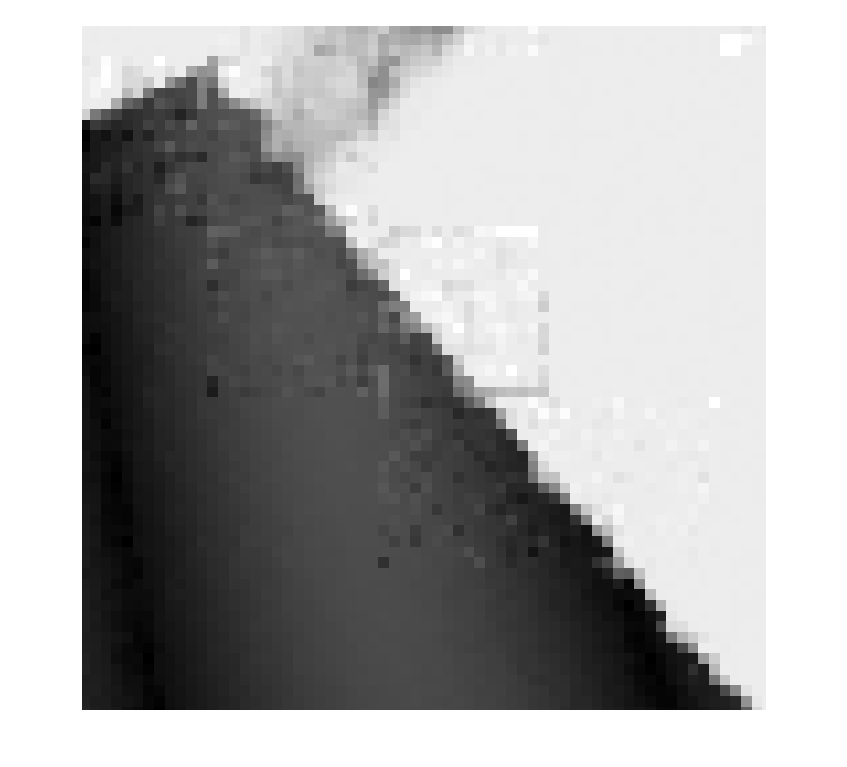
\includegraphics[width=\columnwidth]{images/framing_artifacts.png}
\caption{Artifacts occur w/o frames (left) that vanish with frames (right).} % TODO
\label{framing_artifacts}
\end{figure}

\item For obtaining an initial reconstruction of the image, we compute a weighted sum over all the neighboring pixels that are known. By setting all unknown pixels in the image to zero and encoding known values with 1s in the mask, elementwise division of the filtered image by the similarly filtered mask results in a normalized sum weighted by the filtering kernel.\\
This procedure, which we call Gaussian interpolation, allows us to use MATLAB's fast native functions and to fill holes up to the kernel size, which is another global parameter.
\label{gaussian_interpolation}
\end{enumerate}

After these preparing steps, we start to iteratively improve the reconstructed image with the following steps:
\begin{enumerate}
\item Using the above mentioned validation set, we evaluate several thresholds for every patch and keep for each the best one: After calculating a Fourier transform for every patch, frequencies weaker then the threshold are suppressed by setting them to 0. Since profiling showed that the Fourier transform with its inverse is by far the most time-consuming part of our algorithm, we try to perform as few threshold evaluations as possible. For this purpose, we iteratively evaluate two new thresholds around a center threshold, taking the best one as the new center and halve the step size (see figure \ref{threshold_optimization}). While this heuristic does not always reach the minimum, it works quite well for our error function, which is often roughly convex. For this optimization as well as for the whole iteration, we have both a number- and a convergence-based termination criterion.

\begin{figure}
\centering
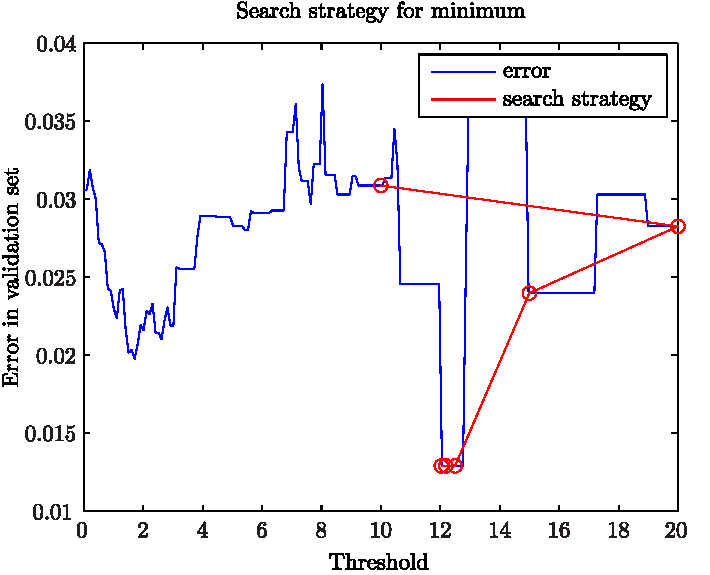
\includegraphics[width=0.8\columnwidth]{../plots/search_strategy_6.pdf}
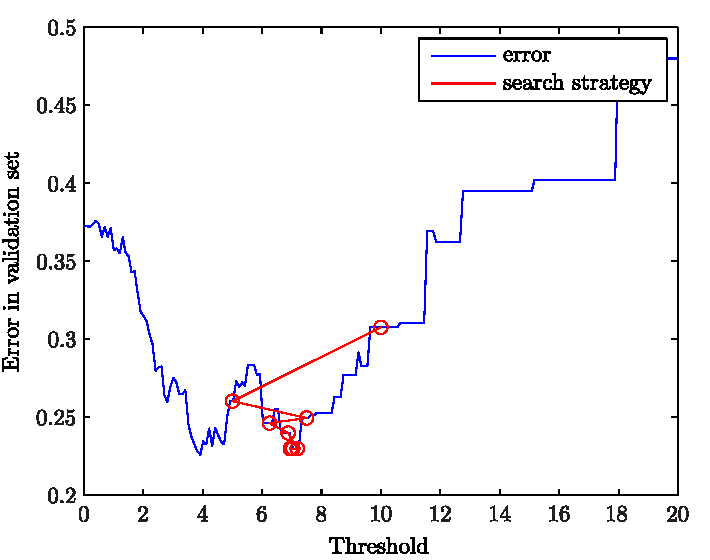
\includegraphics[width=0.8\columnwidth]{../plots/search_strategy_2.pdf}
\caption{The threshold is optimized by iteratively.}
\label{threshold_optimization}
\end{figure}

\item Having stored the reconstruction of every patch with its best threshold, all that remains to do is copying the newly estimated missing pixels (including those of the validation set) back into the reconstructed image.
\end{enumerate}
Finally, the frame added in the beginning is removed again and the pixels of the validation set are overwritten by the original ones. A variant of the presented method is to do it non-iteratively and revert to the original data after determining the thresholds, such that the Gaussian interpolation and the thresholding in the Fourier space is performed without the validation set.

\subsection{Global parameter optimization}
\subsubsection{Optimized parameters}
As shown in table \ref{parameters}, our algorithm has a total of 10 parameters that can be set globally. Instead of tuning them by hand, we automated the optimization process and implicitly use the best parameters found so far, which we store in the file system. This feature also allows us to interrupt the optimization process at any time and continue with the best parameters later on.

\begin{table*}
\begin{center}
\begin{tabular}{|l|p{6cm}|r|r|}
\hline
Parameter & Description & Initial value & Optimized value\\
\hline
gauss\_size & Size of the Gaussian kernel in pixels & 10 & ? \\
gauss\_sigma & Sigma of the Gaussian kernel & 1 & ? \\
patch\_size & Patch size as exponent to the basis 2 & 4 & ? \\
patch\_frame\_size & Frame size in pixels & 8 & ? \\
td\_abortbelow\_stdev & Minimal standard deviation while evaluating thresholds as negative exponent to basis 10& 3 & ? \\
td\_abortbelow\_stepsize & Minimal step size while evaluating thresholds as negative exponent to basis 10& 4 & ? \\
td\_middle & Initial threshold & 10 & ? \\
validation & Fraction of pixels in the validation set & 0.4 & ? \\
max\_iterations & Maximum number of iterations & 5 & ? \\
abortbelow\_change & Minimal relative change to perform another iteration & 0.1 & ? \\
\hline
\end{tabular}
\end{center}
\caption{Parameters with their initial and optimized values.}
\label{parameters}
\end{table*}

\subsubsection{Gradient descent}
\label{gradient_descent}
We optimize all parameters at once using a gradient descent method. Since our cost function is based on measurements, we cannot derive it with respect to individual parameters and have to determine the gradient with finite differences. Besides weighting the parameters with respect to their improvements (which gives us the slope), we also defined a momentum term of 0.8 that should help us to overcome local minima and improve convergence speed. Figure \ref{gradient_descent_cost} shows the development of the cost for 100 optimization steps.

\begin{figure}
\centering
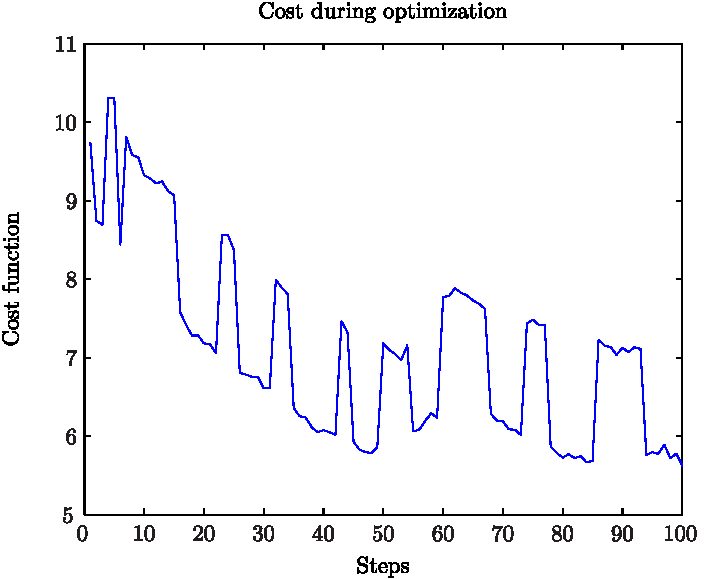
\includegraphics[width=0.8\columnwidth]{../plots/cost_plot.pdf}
\caption{Due to the momentum term, the cost function does not strictly decrease when optimizing.}
\label{gradient_descent_cost}
\end{figure}

\subsubsection{Cost function}
For optimizing a set of parameters, a cost function is needed. Its most important component is obviously the error function used in the submission system, which calculates the mean over the squared differences between the reconstructed and the original image. However, without including the performance of the algorithm, the runtime could grow arbitrarily to get the best accuracy possible. We considered several cost functions based on the error $E$ and the time $T$ (see table \ref{cost_functions}). These two values are scaled appropriately: Usually, the error is multiplied by a factor of 10'000 and the time (measured in seconds) by a factor of 0.01.

\begin{table*}
\centering
{\renewcommand{\arraystretch}{1.5}
\renewcommand{\tabcolsep}{0.2cm}
\begin{tabular}{|l|p{6cm}|p{6cm}|}
\hline
Function & Advantages & Disadvantages \\
\hline
$E + T$ & Easy to understand and everywhere a good gradient & Linear improvement does not necessarily follow one's intuition about the ordering of results \\
\hline
$\exp(E)+\exp(T)$ & Fast increase for both error and time & Not enough gradient for very low $E$ and $T$ values \\
\hline
$(1-\exp(E))*(1-\exp(T))$ & Allows very large times for very low errors & Also true vice versa, i.e. a minimization in time \\
\hline
$ \begin{cases}
E & \text{if }T<T_0\\
E+\exp(T/T_0 - 1) - 1 & \text{otherwise}
\end{cases} $ & Continuous function, optimizes for error when the time is below a target time $T_0$, penalizes long times. & Seems to work quite well, used by us \\
\hline
\end{tabular}}
\caption{Various cost functions used in the optimization process.}
\label{cost_functions}
\end{table*}

\subsubsection{Sample data}
We used the three images provided for the last exercise and four additional ones (consisting of both natural and artificial images, see figure \ref{new_images}) to evaluate the accuracy and performance of the chosen parameters. Instead of using the supplied mask, however, we generate one randomly for every evaluation in order to prevent overfitting to a particular mask.

\begin{figure*}
  \centering
  \subfloat{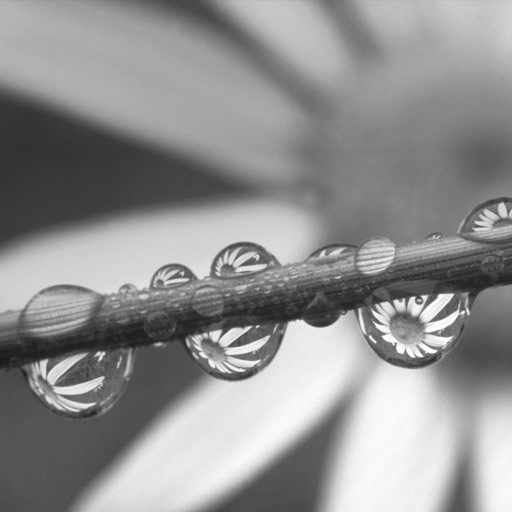
\includegraphics[width=0.24\textwidth]{../daisiesFromBing512x512}}~
  \subfloat{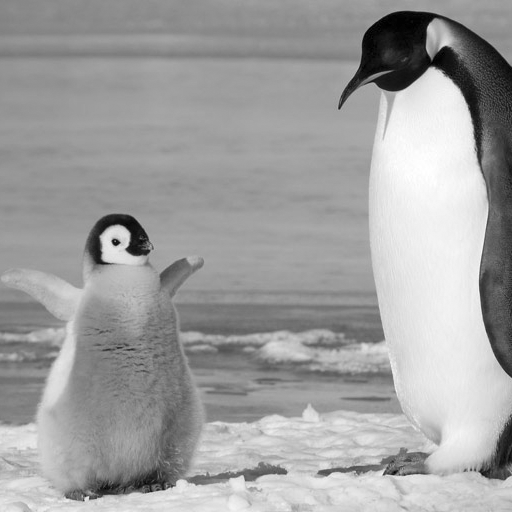
\includegraphics[width=0.24\textwidth]{../penguinsFromBing512x512}}~
  \subfloat{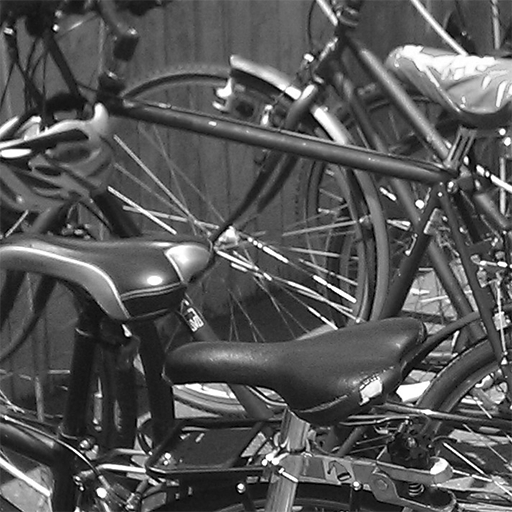
\includegraphics[width=0.24\textwidth]{../velos512x512}}~
  \subfloat{
\includegraphics[width=0.24\textwidth]{../hardedges_512x512}}~
  \caption{The four additional images used during optimization.}
  \label{new_images}
\end{figure*}

\subsubsection{Found values}
Our observations during the optimization process can be split into three classes:
\begin{itemize}
\item Some parameters converged towards their estimated value. The size of the Gaussian kernel, for example, has to be slightly bigger than the largest hole assumed in an image.
\item Some parameters have a clear speed vs. accuracy tradeoff, like the stopping conditions of the threshold optimization, which depend on our cost function and could not be foreseen.
\item Some parameters assumed totally different values than anticipated: The patch size became much larger and the validation set decreased significantly, as can be seen in figure \ref{gradient_descent_parameters}.
\end{itemize}

\begin{figure}
  \centering
  \subfloat{\label{fig:gull}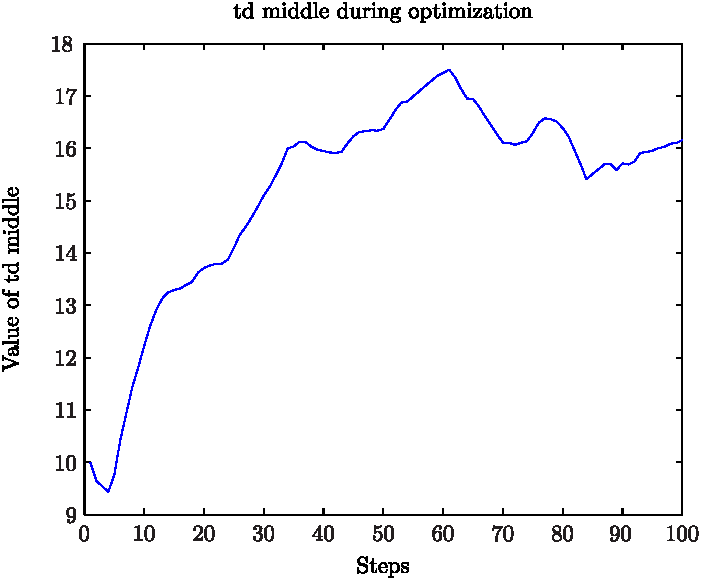
\includegraphics[width=0.25\textwidth]{../plots/td_middle_plot.pdf}}                
  \subfloat{\label{fig:tiger}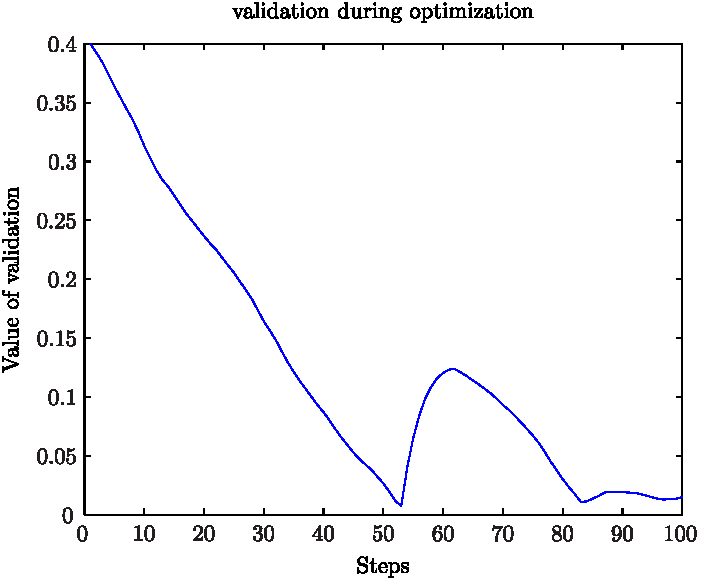
\includegraphics[width=0.25\textwidth]{../plots/validation_plot.pdf}}
  \caption{Two parameters that seem to converge quite well during the optimization.}
  \label{gradient_descent_parameters}
\end{figure}

\section{Results}
We compared our algorithm with the following three baseline algorithms (see figure \ref{baseline_algorithms}):
\begin{enumerate}
\item Vertical and horizontal linear interpolation,
\item Gaussian interpolation as described in section \ref{gaussian_interpolation} and
\item Matching pursuit~\cite{matchingpursuit93} with an overcomplete dictionary of discrete cosines.
\end{enumerate}

\begin{figure}
\centering
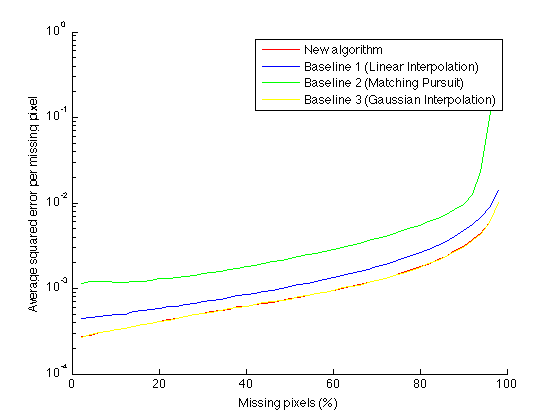
\includegraphics[width=\columnwidth]{images/missingpixelsVsError.png}
\caption{Baseline algorithms for various fractions of missing pixels.}
\label{baseline_algorithms}
\end{figure}
 
We evaluated the baseline algorithms with the same sample images as optimization. With 60\% missing pixels, the algorithms had the following errors and standard deviations:

\begin{table}[h]
\centering
\begin{tabular}{l|r|r}
Algorithm & Error & Deviation \\
\hline
Linear interpolation & ? & ? \\
Gaussian interpolation & ? & ? \\
Matching pursuit & ? & ? \\
\end{tabular}
\end{table}

Our algorithm did not perform equally well for all sample images: It worked best for ? (error ? and standard deviation ?) and worst for ? (error ? and standard deviation ?).

The strength of our method is definitely in reconstructing edges, which can be seen in figure \ref{edge_reconstruction}.

\begin{figure}
\centering
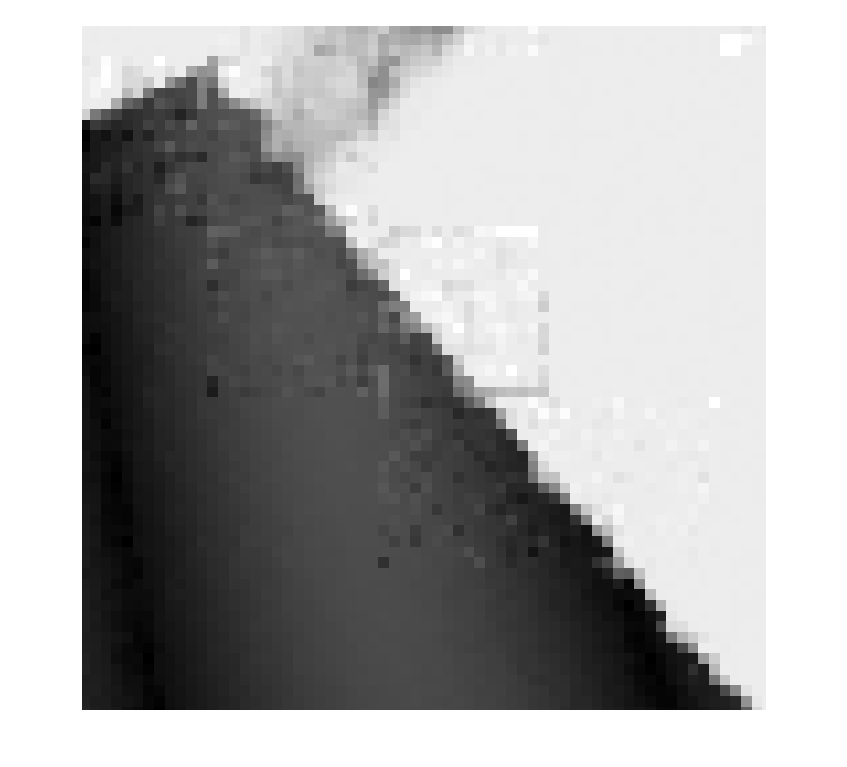
\includegraphics[width=\columnwidth]{images/framing_artifacts.png}
\caption{Original image with mask (left) and its reconstruction (right).}
\label{edge_reconstruction}
\end{figure}

\paragraph{Note} All plots in this paper were created with MATLAB and were produced using the script \emph{CreatePaperPlots.m} of our submission. However, due to the randomness of the algorithm and varying speed measurements for the cost function, results can be different for each run.

\section{Discussion}
Discuss the strengths and weaknesses of your approach, based on the results. Point out the implications of your novel idea on the application concerned. TODO

\section{Summary}
Making use of our domain knowledge about images, we have implemented an algorithm that performs well in terms of both accuracy and performance. The remarkable speed is achieved by relying on MATLAB's native functions for the most computationally intensive tasks. In our opinion, we have devised many nice methods: Gaussian interpolation, threshold optimization with validation set and frequency suppression in the Fourier domain to name just the most important ones. The key feature of our algorithm is certainly its ability to reconstruct the edges in an image.

\section*{Acknowledgements}
Our implementation is based on the inpainting and evaluation framework provided by the course \emph{Computer Intelligence Lab} held by Prof. Joachim Buhmann at ETH Zurich.

\bibliographystyle{IEEEtran}
\bibliography{biblio}

\end{document}
